\section{Experimental Results}
This chapter gives an overview of the experimental setup, applied metrics
(\cref{sect:metrics}), and data sets (\cref{sect:staver,sect:tkstede}). Summary
and conclusion are given in \cref{sect:results-and-discussion}.

\subsection{Metrics}\label{sect:metrics}
To evaluate and compare approaches described in \cref{chap:Methodology} we
discuss a set of metrics in this section. We consider
\nameref{subsect:pixel-wise-metrics}, \nameref{subsect:mAP} and also
introduce \nameref{subsect:normalized-iou}.

\subsubsection{Pixel-wise Metrics}\label{subsect:pixel-wise-metrics}
In this subsubsection we briefly explain pixel-wise metrics such as
\nameref{par:precision-recall}, \nameref{par:f-scores} and \nameref{par:iou}.

\paragraph{Precision \& Recall}\label{par:precision-recall}
To the best of our knowledge, the most influential metric used in stamp 
detection is pixel-wise evaluation of the Precision and Recall
tuple~\cite{Nandedkar.2015121620151219,Younas.2017110920171115,
Ahmed.2013082520130828,Dey.2015121620151219,
Micenkova.2011091820110921, Bhalgat.20160916, Micenkova.2015,
Nandedkar.2015082320150826}. Often, recall and precision are used in settings
with class imbalance where they provide a more sensible measure than accuracy.
In the stamp detection, every image pixel one can consider two classes, either
\textit{stamp} or \textit{non-stamp}. In training and evaluation images,
\textit{non-stamp}-pixels greatly outnumber \textit{stamp}-pixels. Therefore,
showing obvious class imbalance.
\par
A definition of precision and recall is given
in~\cite[423]{Goodfellow.2016} as the fraction of 
\glsdisp{tp}{\textit{true} positive (TP)} detections over positive detections (i.e.\ \glspl{tp} and \glspl{fp}) and the
fraction of \glsdisp{tp}{\textit{true} positive} detections over positive \textit{datapoints}
(i.e.\ \glspl{tp} and \glspl{fn}):
\begin{align}
    \text{Precision} &= \frac{TP}{TP + FP}\\
    \text{Recall} &= \frac{TP}{TP + FN}\label{eq:precision-recall}
\end{align}
Intuitively, precision is the ``ability of a classifier to distinguish a
negative sample from [a] positive one''~\cite{Younas.2017110920171115}, while
recall is ``the ability of a classifier to classify all positive samples''~\cite{Younas.2017110920171115}.
A visual example of recall and precision is given in
\cref{fig:visual-precision-recall}.
\begin{figure}
    \center
    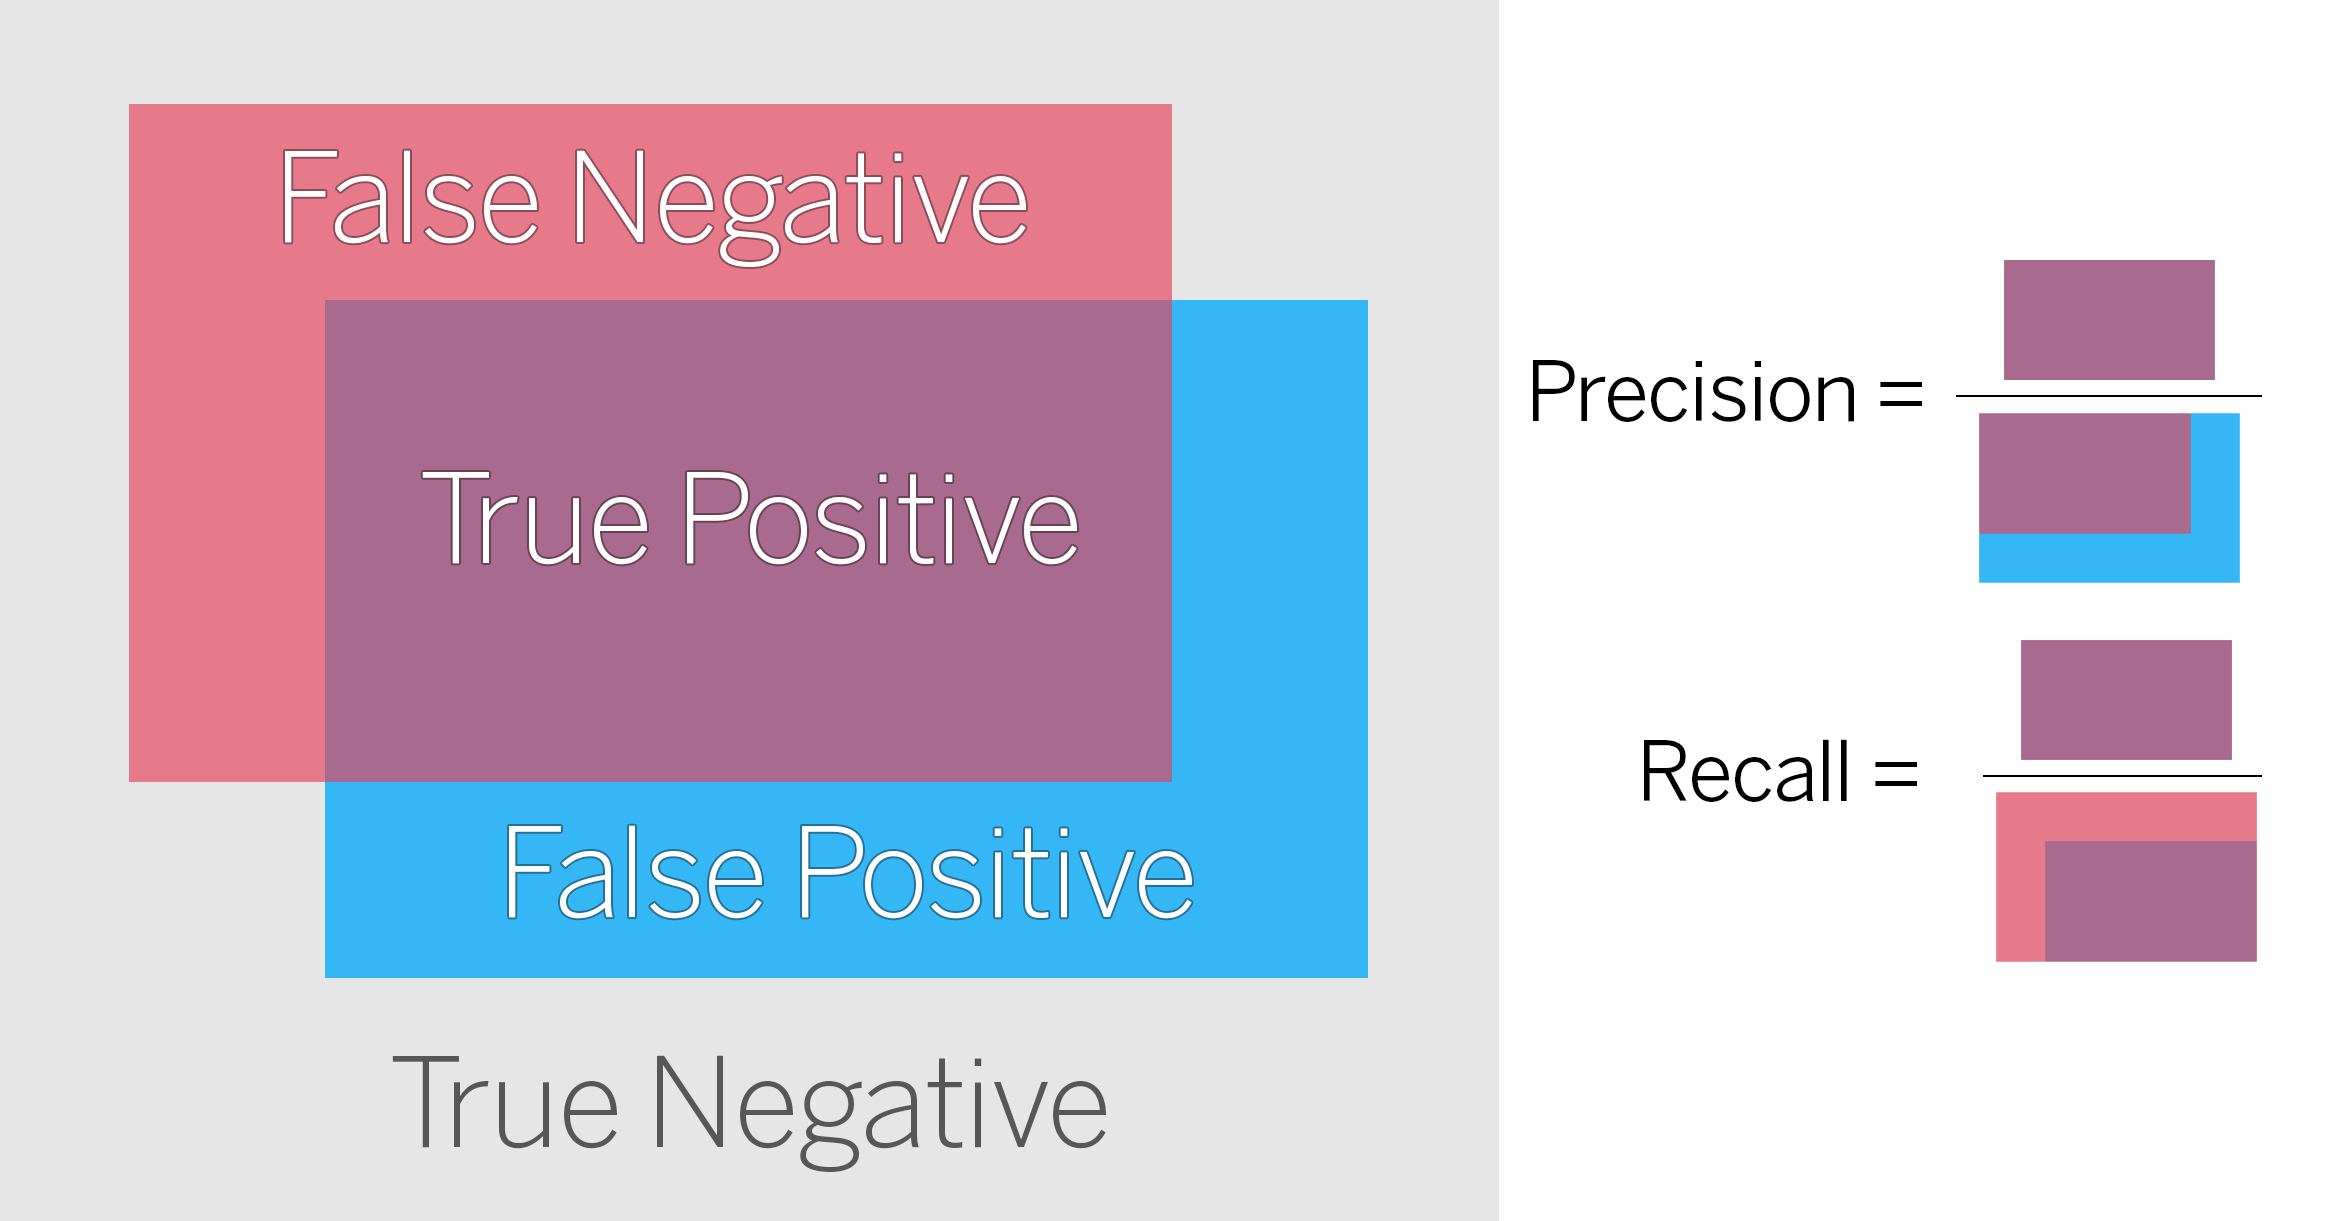
\includegraphics[width=\textwidth]{Metrics2.png}
    \caption[short={Visual example of pixel-wise recall, precision and \gls{iou}}]
    {Visual example of pixel-wise recall, precision and \gls{iou}, with
    groundtruth (red) and inferred detection (blue)}\label{fig:visual-precision-recall}
\end{figure}

\paragraph{F-Scores}\label{par:f-scores}
Precision and Recall can then be combined into a single harmonic average: the
family of \(F_\beta\)-Scores. \(F_1\) is given in~\cite[424]{Goodfellow.2016} as
\begin{equation*}
    F_1=\frac{2*\text{Precision}*\text{Recall}}{\text{Precision} + \text{Recall}}
\end{equation*}
However, almost all works give only Precision \& Recall and omit F-Scores.

\paragraph{Intersection over Union}\label{par:iou}
\Gls{iou}, also known as the Jaccard-Index or Jaccard Similarity is a metric
closely related to \nameref{par:f-scores} via the Tversky-Index (for details on
this \cite[cf.][Section 6.3 Similarity Measures]{James.2011}). \Gls{iou} is 
given by
\begin{equation}
    \text{IoU}=\frac{TP}{TP + FN + FP}
\end{equation}
Visually, this relation is shown in \cref{fig:visual-precision-recall}.

\subsubsection{Class-wise Mean Average Precision}\label{subsect:mAP}
\Gls{map} is a widely used metric in object detection that was also adopted in
challenges such as \gls{coco}, \gls{voc}, and \gls{oi}. We define \gls{map} in
context of a multi-classification setting, where \gls{map} represents the
arithmetic mean of \gls{ap} over the set of all classes. Next up we will
redefine confusion matrix-values, then average precision will be explained.

\paragraph{Confusion Matrix}
Unlike in \fref{subsect:pixel-wise-metrics}, confusion matrix-values
(\glspl{tp}, \glspl{fp} \& \glspl{fn}) are attributed not per individual pixel,
but per \gls{bbox}. A predicted \gls{bbox} is considered a \gls{tp}, if its
(pixel-wise) \gls{iou} with a groundtruth \gls{bbox} is greater than some
threshold, \gls{fp} otherwise. Groundtruth \glspl{bbox} without an inferred
\gls{bbox} are considered \gls{fn}.
\par
For example assume minimum \gls{iou}\(=0.5\). Then, in
\cref{fig:bbox-precision-recall} \glspl{bbox} \(A\) and \(B\) would be considered
\glspl{fp} due to their low \gls{iou}, while \gls{bbox} \(B\) is a \gls{tp}.
We count 1 \gls{tp}, 2 \gls{fp} and 1 \gls{fn} and thus observe
\(\text{Precision} = \frac{1}{3}, \text{Recall} = \frac{1}{2}\), following
\cref{eq:precision-recall}.

\begin{figure}
    \center
    \includegraphics[width=\textwidth/4]{metrics3.png}
    \caption{Visual example for bounding-box-wise confusion matrix, with
    groundtruth \glspl{bbox} (red) and inferred \glspl{bbox}(blue). For each
    inferred \gls{bbox} a confidence score (percent) is given.}\label{fig:bbox-precision-recall}
\end{figure}

\paragraph{Precision-Recall-Curves and Average Precision}\label{par:precision-recall-curves-ap}
By ordering set of inferred \glspl{bbox} by confidence and then accumulating
\glspl{tp} and \glspl{fp}, we can construct a Precision-Recall-Curve.
A more extensive example is shown in \cref{fig:precision-recall-curve}.
To improve comparability, a curve \(f(x)\) can be smoothed by applying
\(f(x) = \max (f(x), f(x')), \forall x' > x\). 

\begin{figure}[!tpb]
    \center
    \subfloat[Precision-Recall-Curve. Each capital represents an inferred
    \gls{bbox}. Recall \& Precision are plotted by accumulating \gls{tp} and
    \gls{fp} over the list of inferred \glspl{bbox} sorted by confidence.] {
        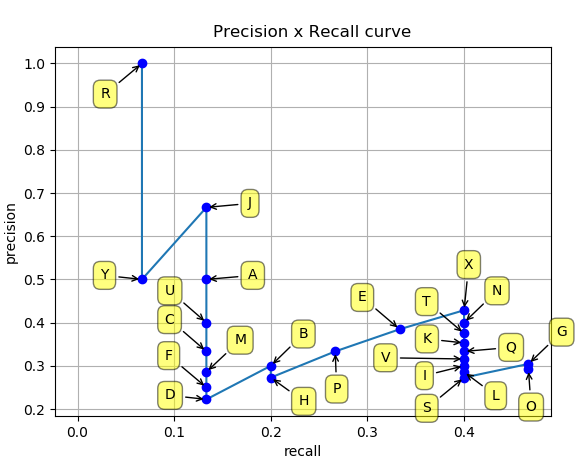
\includegraphics[width=\textwidth/2]{rafaelpadilla-precision-recall-curve.png}
    }
    \subfloat[Interpolated Precision-Recall-Curve with drawn-in area under the
    curve, i.e.\ \gls{ap}.]{
        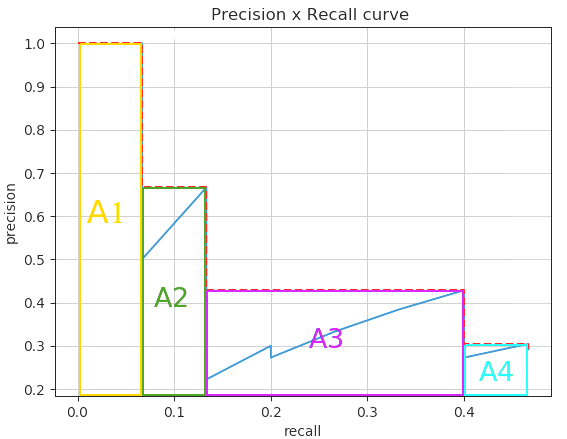
\includegraphics[width=\textwidth/2]{rafaelpadilla-average-precision.png}
    }
    \caption[short={Precision-Recall-Curve}]{Precision-Recall-Curve and its
    interpolation. Both figures where adopted from~\cite{Padilla.2019}}
    \label{fig:precision-recall-curve}
\end{figure}

\Gls{map} builds upon \gls{ap}. \Gls{ap} is a 
Despite its extensive use in the object detection community~\cite{Liu.2016,Ren.20150604}, 
\Gls{map} was only applied in a single work \cite{Zhu.2006} from 2006. This is,
because 
\begin{enumerate*}[i.)]
    \item usually ranks are not generated in most approaches, therefore the 
    underlying metric of average precision, which \textit{is} computed over ranks, 
    lacks meaning and
    \item oftentimes stamp detection is framed as a binary problem.
\end{enumerate*} 

\subsubsection{Normalized Intersection Over Union}\label{subsect:normalized-iou}
\blindtext[1]
\todo{This kind of has the same issues as accuracy. Imagine, 99\% of images are
in the lower left corner, the a System that learns this would have a high 
average IoU. Maybe combine this from ideas of the F-Score.}

\subsection{StaVer}\label{sect:staver}
``The presented method is evaluated on a publicly available dataset (StaVer1) for stamp
detection and verication [sic!]. This dataset contains 400 scanned document images. Out
of these 400 documents, 80 documents contain black stamps whereas the remaining 320
documents contain colored stamps. All of these document images are available in 200,
300, and 600 dpi. For each image, two different types of ground truths are available.
One contains the pixel level ground truth, which means all of the pixels which belong to
stamps are marked in the image. The other ground truth format contains bounding box
information for each stamp. Hence, this dataset can be used for both pixel level as well
as patch level evaluation of stamp detection. In addition, it contains different types of
stamps ranging from rectangular, oval, to irregular shaped, and most importantly, textual
stamps.
For evaluation of the presented approach, the training set is generated by using 36 documents
out of 400. Out of these 36 training documents, only 6 contains black stamps
whereas the remaining 30 are with colored stamps. Testing is performed on the remaining
364 documents (74 documents with black stamps, 290 documents with colored stamps).
All the results are reported for 200 dpi documents.''~\cite{Ahmed.2016}

\subsection{Results \& Discussion}\label{sect:results-and-discussion}
Goals: 
    a.) How good can stamp detection get with current frameworks
    b.) How good can classification of a vast variety of similar classes get
        with current frameworks